\documentclass[../main.tex]{subfiles}
\begin{document}

% En compilation individuelle, la mention légale est affichée.
% Dans le livre complet, elle figure déjà sur la page de garde.
\ifSubfilesClassLoaded{\PageLegaleChapitre}{}

\chapter{Trigonométrie dans le triangle rectangle}
\label{chap:trigonometrie}

% =====================================================
\section{Le triangle rectangle et la terminologie}
% =====================================================

La trigonométrie (du grec \textit{trigonon}, « triangle », et \textit{metron}, « mesure ») étudie les relations entre les longueurs des côtés et les angles d'un triangle. En 3\textsuperscript{e} secondaire, on débute dans le \textbf{triangle rectangle}, c'est-à-dire un triangle qui possède un angle de $90^\circ$.

\subsection{Nommer les côtés par rapport à un angle}

Dans un triangle rectangle, les côtés portent des noms précis selon l'angle aigu $\alpha$ que l'on étudie :

\begin{center}
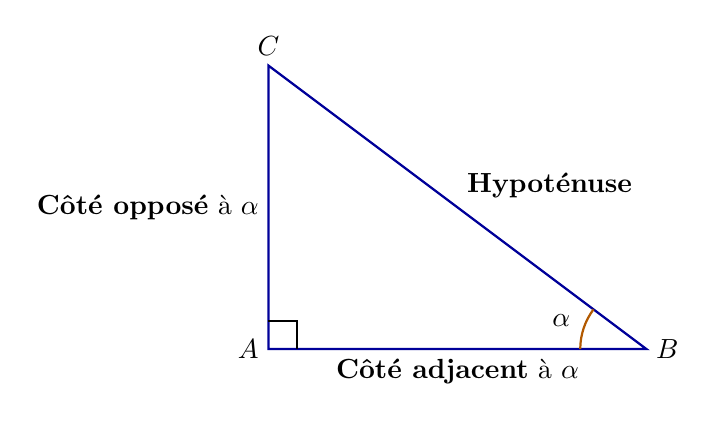
\begin{tikzpicture}[scale=1.2]
  % Sommets du triangle
  \coordinate (A) at (0,0);
  \coordinate (B) at (4,0);
  \coordinate (C) at (0,3);

  % Tracé du triangle
  \draw[thick, blue!60!black] (A) -- (B) -- (C) -- cycle;

  % Angle droit en A
  \draw[thick] (0.3,0) -- (0.3,0.3) -- (0,0.3);

  % Étiquettes des sommets
  \node[left] at (A) {$A$};
  \node[right] at (B) {$B$};
  \node[above] at (C) {$C$};

  % Étiquettes des côtés
  \node[below] at (2,0) {\textbf{Côté adjacent} à $\alpha$};
  \node[left] at (0,1.5) {\textbf{Côté opposé} à $\alpha$};
  \node[above right] at (2,1.5) {\textbf{Hypoténuse}};

  % Arc de l'angle alpha en B
  \draw [thick, orange!70!black] (3.3,0) arc (180:143.13:0.7);
  \node at (3.1,0.3) {$\alpha$};
\end{tikzpicture}
\end{center}

\begin{definition}
Soit un triangle rectangle.
\begin{itemize}
  \item L'\textbf{hypoténuse} est le côté le plus long. C'est toujours celui qui se trouve \textbf{en face de l'angle droit}. Elle ne change jamais de place.
  \item Le \textbf{côté opposé} à l'angle $\alpha$ est le côté situé \textbf{en face} de cet angle.
  \item Le \textbf{côté adjacent} à l'angle $\alpha$ est le côté qui \textbf{touche} cet angle, sans être l'hypoténuse.
\end{itemize}
\end{definition}

\begin{attention}
Les côtés opposé et adjacent dépendent de l'angle $\alpha$ que l'on regarde. Si l'on change d'angle aigu dans le même triangle, leurs rôles s'inversent.
\end{attention}

% =====================================================
\section{Les trois rapports trigonométriques}
% =====================================================

Dans un triangle rectangle, le rapport entre deux côtés ne dépend que de la mesure de l'angle aigu, et pas de la taille du triangle. On définit ainsi le \textbf{sinus}, le \textbf{cosinus} et la \textbf{tangente}.

\begin{propriete}[Formules fondamentales -- SOH CAH TOA]
Pour un angle aigu $\alpha$ dans un triangle rectangle :
\[
\sin(\alpha) = \frac{\text{côté opposé}}{\text{hypoténuse}} \quad (\textbf{SOH}), \qquad
\cos(\alpha) = \frac{\text{côté adjacent}}{\text{hypoténuse}} \quad (\textbf{CAH}),
\]
\[
\tan(\alpha) = \frac{\text{côté opposé}}{\text{côté adjacent}} \quad (\textbf{TOA}).
\]
\end{propriete}

\textbf{Astuce mnémotechnique :} retiens le mot \textbf{SOH-CAH-TOA}.
\begin{itemize}
  \item \textbf{S}in = \textbf{O}pposé / \textbf{H}ypoténuse
  \item \textbf{C}os = \textbf{A}djacent / \textbf{H}ypoténuse
  \item \textbf{T}an = \textbf{O}pposé / \textbf{A}djacent
\end{itemize}

\subsection{Quelques valeurs à connaître}

\begin{center}
\renewcommand{\arraystretch}{1.5}
\begin{tabular}{|c|c|c|c|}
\hline
$\alpha$ & $30^\circ$ & $45^\circ$ & $60^\circ$ \\ \hline
$\sin(\alpha)$ & $\dfrac{1}{2}$ & $\dfrac{\sqrt{2}}{2}$ & $\dfrac{\sqrt{3}}{2}$ \\ \hline
$\cos(\alpha)$ & $\dfrac{\sqrt{3}}{2}$ & $\dfrac{\sqrt{2}}{2}$ & $\dfrac{1}{2}$ \\ \hline
$\tan(\alpha)$ & $\dfrac{\sqrt{3}}{3}$ & $1$ & $\sqrt{3}$ \\ \hline
\end{tabular}
\end{center}

% =====================================================
\section{Utilisations pratiques}
% =====================================================

\subsection{Calculer la longueur d'un côté}

\begin{methode}
\begin{enumerate}
  \item Repérer l'angle connu et identifier les côtés concernés (opposé, adjacent ou hypoténuse).
  \item Choisir le rapport trigonométrique adéquat ($\sin$, $\cos$ ou $\tan$).
  \item Poser l'équation et isoler l'inconnue (produit en croix).
\end{enumerate}
\end{methode}

\textbf{Exemple.} Dans un triangle rectangle, $\alpha = 30^\circ$, l'hypoténuse vaut $10$ cm et on cherche le côté opposé $x$ :
\[
\sin(30^\circ) = \frac{x}{10} \quad\Longrightarrow\quad x = 10 \times \sin(30^\circ) = 10 \times 0\dec 5 = 5 \text{ cm}.
\]

\subsection{Calculer la mesure d'un angle}

\begin{methode}
Quand on connaît deux côtés et que l'on cherche l'angle $\alpha$ :
\begin{enumerate}
  \item Écrire le rapport trigonométrique qui relie les deux côtés connus.
  \item Utiliser la fonction inverse de la calculatrice ($\sin^{-1}$, $\cos^{-1}$ ou $\tan^{-1}$, souvent avec la touche \texttt{2nd} ou \texttt{Shift}).
\end{enumerate}
\end{methode}

\textbf{Exemple.} Si $\tan(\alpha) = \dfrac{3}{4} = 0\dec 75$, alors $\alpha = \tan^{-1}(0\dec 75) \approx 36\dec 87^\circ$.

% =====================================================
\section{Récapitulatif}
% =====================================================

\begin{tcolorbox}[colback=gray!6,colframe=gray!60!black,title={\bfseries À retenir}]
\[
\sin(\alpha) = \frac{\text{opp}}{\text{hyp}}, \qquad \cos(\alpha) = \frac{\text{adj}}{\text{hyp}}, \qquad \tan(\alpha) = \frac{\text{opp}}{\text{adj}}
\]
\textbf{Réflexes :}
\begin{itemize}
  \item Vérifier que la calculatrice est en \textbf{degrés (DEG)} et non en radians.
  \item L'hypoténuse est toujours plus grande que les deux autres côtés : le sinus et le cosinus d'un angle aigu sont donc toujours compris entre $0$ et $1$.
  \item Toujours nommer les côtés (opposé, adjacent, hypoténuse) \textbf{avant} de choisir la formule.
\end{itemize}
\end{tcolorbox}

\newpage
% =====================================================
\section{Exercices}
% =====================================================

\subsection{Série A -- Briefing au sol : identification et application directe}

\begin{enumerate}[label=\textbf{\arabic*.}]

\item Dans un triangle $ABC$ rectangle en $A$, écris les formules de $\sin(B)$, $\cos(B)$ et $\tan(B)$ en fonction des côtés du triangle.

\item Calcule la valeur arrondie au centième (vérifie bien le mode de ta calculatrice) :
\begin{enumerate}[label=\alph*)]
  \item $\sin(45^\circ)$ \qquad
  \item $\cos(60^\circ)$ \qquad
  \item $\tan(30^\circ)$ \qquad
  \item $\sin(72^\circ)$
\end{enumerate}

\item Le pilote lit ses instruments : trouve l'angle $\alpha$ au dixième de degré près.
\begin{enumerate}[label=\alph*)]
  \item $\sin(\alpha) = 0\dec 5$ \qquad
  \item $\cos(\alpha) = 0\dec 8$ \qquad
  \item $\tan(\alpha) = 2$ \qquad
  \item $\sin(\alpha) = \dfrac{3}{5}$
\end{enumerate}

\end{enumerate}

\subsection{Série B -- Carnet de campagne : longueurs et angles}

\begin{enumerate}[label=\textbf{\arabic*.},start=4]

\item Le triangle $RST$ est rectangle en $S$, avec $\widehat{T} = 40^\circ$ et $RT = 12$ cm. Calcule la longueur du côté $ST$ (adjacent à $\widehat{T}$).

\item Le triangle $MNP$ est rectangle en $N$. Le côté opposé à l'angle $\widehat{M}$ mesure $5$ cm et le côté adjacent mesure $7$ cm. Calcule la mesure de l'angle $\widehat{M}$.

\item Un éclaireur appuie une perche de $6$ m contre un mur vertical pour monter un abri. Le pied de la perche est à $2$ m du mur. Quel angle la perche forme-t-elle avec le sol ?

\end{enumerate}

\subsection{Série C -- Missions de vol et de camp}

\textbf{Mission 1 -- Approche à l'atterrissage.}
Un avion de ligne descend selon une pente de $3^\circ$ par rapport à l'horizontale.
\begin{enumerate}[label=\alph*)]
  \item À $10$ km de la piste (distance mesurée au sol), à quelle altitude doit-il se trouver ? Donne le résultat en mètres, arrondi à l'unité.
  \item Il se trouve à $3\,000$ m d'altitude. À quelle distance horizontale de la piste doit-il commencer sa descente ? Donne le résultat en km, arrondi au dixième.
\end{enumerate}

\textbf{Mission 2 -- Montée initiale.}
Après le décollage, un avion monte avec un angle de $15^\circ$ par rapport au sol et parcourt $3\,000$ m le long de sa trajectoire. Quelle altitude a-t-il gagnée ? Quelle distance horizontale a-t-il parcourue ? (arrondis à l'unité)

\textbf{Mission 3 -- Hauteur d'un arbre.}
Pour estimer la hauteur d'un arbre, un éclaireur se place à $20$ m de son pied. Il vise le sommet avec un angle de $35^\circ$ au-dessus de l'horizontale. Ses yeux sont à $1\dec 5$ m du sol. Quelle est la hauteur de l'arbre (au dixième de mètre) ?

\textbf{Mission 4 -- Tyrolienne.}
Un câble de $40$ m relie deux arbres dont les points d'attache ont $8$ m de dénivelé. Quel angle le câble forme-t-il avec l'horizontale (au dixième de degré) ?

\textbf{Mission 5 -- L'ombre du mât.}
Le soleil est à $40^\circ$ au-dessus de l'horizon. Le mât de drapeau du camp mesure $6$ m. Quelle est la longueur de son ombre au sol (au centième de mètre) ?

\subsection{Défi bonus}

\begin{enumerate}[label=\alph*)]
  \item Démontre que, pour tout angle aigu $\alpha$ d'un triangle rectangle, $\tan(\alpha) = \dfrac{\sin(\alpha)}{\cos(\alpha)}$.
  \item Sachant que $\sin^2(\alpha) + \cos^2(\alpha) = 1$, calcule $\cos(\alpha)$ si $\sin(\alpha) = 0\dec 6$.
\end{enumerate}

\newpage
% =====================================================
\section{Corrigés}
% =====================================================

\subsection*{Série A}

\textbf{1.} $\sin(B) = \dfrac{\text{opposé}}{\text{hypoténuse}} = \dfrac{AC}{BC}$, \quad $\cos(B) = \dfrac{\text{adjacent}}{\text{hypoténuse}} = \dfrac{AB}{BC}$, \quad $\tan(B) = \dfrac{\text{opposé}}{\text{adjacent}} = \dfrac{AC}{AB}$.

\textbf{2.} a) $0\dec 71$ \quad b) $0\dec 5$ \quad c) $0\dec 58$ \quad d) $0\dec 95$

\textbf{3.} a) $\alpha = 30^\circ$ \quad b) $\alpha \approx 36\dec 9^\circ$ \quad c) $\alpha \approx 63\dec 4^\circ$ \quad d) $\alpha \approx 36\dec 9^\circ$

\subsection*{Série B}

\textbf{4.} Le côté $ST$ est adjacent à $\widehat{T}$ et on connaît l'hypoténuse $RT$ : on utilise le cosinus.
\[
\cos(40^\circ) = \frac{ST}{12} \quad\Longrightarrow\quad ST = 12 \times \cos(40^\circ) \approx 12 \times 0\dec 766 \approx 9\dec 19 \text{ cm}.
\]

\textbf{5.} On utilise la tangente :
\[
\tan(\widehat{M}) = \frac{5}{7} \approx 0\dec 7143 \quad\Longrightarrow\quad \widehat{M} = \tan^{-1}(0\dec 7143) \approx 35\dec 5^\circ.
\]

\textbf{6.} La perche est l'hypoténuse ($6$ m) et la distance au mur est le côté adjacent à l'angle $\alpha$ cherché :
\[
\cos(\alpha) = \frac{2}{6} = \frac{1}{3} \quad\Longrightarrow\quad \alpha = \cos^{-1}\!\left(\frac{1}{3}\right) \approx 70\dec 5^\circ.
\]

\subsection*{Série C}

\textbf{Mission 1.}
\begin{enumerate}[label=\alph*)]
  \item L'altitude est le côté opposé, la distance au sol est le côté adjacent : $\tan(3^\circ) = \dfrac{h}{10\,000}$, donc $h = 10\,000 \times \tan(3^\circ) \approx 524$ m.
  \item $\tan(3^\circ) = \dfrac{3\,000}{d}$, donc $d = \dfrac{3\,000}{\tan(3^\circ)} \approx 57\,243$ m $\approx 57\dec 2$ km.
\end{enumerate}

\textbf{Mission 2.} La trajectoire est l'hypoténuse.
Altitude : $3\,000 \times \sin(15^\circ) \approx 776$ m. \quad Distance horizontale : $3\,000 \times \cos(15^\circ) \approx 2\,898$ m.

\textbf{Mission 3.} $20 \times \tan(35^\circ) \approx 14\dec 0$ m, puis on ajoute la hauteur des yeux : $14\dec 0 + 1\dec 5 = 15\dec 5$ m.

\textbf{Mission 4.} $\sin(\alpha) = \dfrac{8}{40} = 0\dec 2$, donc $\alpha = \sin^{-1}(0\dec 2) \approx 11\dec 5^\circ$.

\textbf{Mission 5.} L'ombre est le côté adjacent à l'angle de $40^\circ$ : $\tan(40^\circ) = \dfrac{6}{\ell}$, donc $\ell = \dfrac{6}{\tan(40^\circ)} \approx 7\dec 15$ m.

\subsection*{Défi bonus}

a) $\dfrac{\sin(\alpha)}{\cos(\alpha)} = \dfrac{\text{opp}/\text{hyp}}{\text{adj}/\text{hyp}} = \dfrac{\text{opp}}{\text{hyp}} \times \dfrac{\text{hyp}}{\text{adj}} = \dfrac{\text{opp}}{\text{adj}} = \tan(\alpha)$.

b) $0\dec 6^2 + \cos^2(\alpha) = 1 \Rightarrow \cos^2(\alpha) = 1 - 0\dec 36 = 0\dec 64 \Rightarrow \cos(\alpha) = \sqrt{0\dec 64} = 0\dec 8$ (positif, car $\alpha$ est aigu).

\end{document}
